% !TeX spellcheck = en_US
\documentclass{toc}
\date{}

%% !!! AUTHOR: Fill in meta-data below
%% Optional items are marked %OPL, followed by explanation "if (when to use)"
%% if using optional item, delete "%OPL"
\tocdetails{%
  title = {Complexity of Linear Operators},
%% please update the following four items when submitting revision
  number_of_pages = {NN},
  number_of_bibitems = {NN},
  number_of_figures = {NN},
  conference_version = {ISAAC19}, %% examples: {EC17},  {FSTTCS18}, {NONE}
  author = {Alexander S. Kulikov, Ivan Mikhailin, Andrey Mokhov, and Vladimir V. Podolskii},
    %% Use the format
    %% "A", or "A and B", or "A, B, and C", or "A, B, C, and D", etc.
    %% e.g., {Author A, Author B, and K\'alm\'an Sz\H{o}l\H{o}ssy},
    %% IMPORTANT: Please use ascii TeX codes for characters with
    %% foreign accents.
  authorlist = {Alexander S. Kulikov, Ivan Mikhailin, Andrey Mokhov, Vladimir V. Podolskii},
    %% Comma separated author list, NO AND: Use the format
    %% "A", or "A, B", or "A, B, C", etc.
    %% NOTE: No "and" at the end--simply comma separated,
    %% e.g., {Author A, Author B, K\'alm\'an Sz\H{o}l\H{o}ssy},
  runningauthor = {A. S. Kulikov, I. Mikhailin, A. Mokhov, V. V. Podolskii},
  copyrightauthor = {Alexander~S. Kulikov, Ivan Mikhailin, Andrey Mokhov, and
    Vladimir V. Podolskii},
  acmclassification = {Theory of computation: Streaming, sublinear and near
    linear time algorithms},
  amsclassification = {Analysis of algorithms and problem complexity (68Q25)},
  keywords = {algorithms, linear operators, commutativity, range queries,
    circuit complexity},  % , lower bounds, upper bounds
    %% keywords and phrases of your choice, lower case, comma separated,
    %% no period at end
    %% please consider using relevant ToC categories -- see
    %%    http://theoryofcomputing.org/categories
    %
}   %% END AUTHOR-FILLED METADATA

%%%%%%%%%%%%%%%%%%%%%%%%%%%%%%%%%%%%%%%%
%%% EDITOR: Fill in meta-data below
\tocdetails{%
%  volume = 1X,      %% example:  volume = 16,
%  number = Y,       %% examples: number = 5,    number = 19,
%  year = 20ZZ,
%  specissue={\cccBH}  %% CCC'17
%  specissue={\cccBI}  %% CCC'18
%  specissue={\cccBJ}  %% CCC'19
%  specissue={\cccCA}  %% CCC'20
%  specissue={\cccCB}  %% CCC'21
%  specissue={\approxrandomBG}  %% APPROX-RANDOM'16
%  specissue={\approxrandomBI}  %% APPROX-RANDOM'18
%  received = {date},
%  revised = {date},
%  published = {date},
%  note,
%  survey,  %% this item refers to "research survey", not "grad survey"
%  exposition, %% refers to "research exposition"
%  doi = {10.4086/toc....},  %% format: doi = {10.4086/toc.2018.v014a009}
}   %% END tocdetails

% \usepackage[utf8]{inputenc}
% \usepackage[english]{babel}
% \usepackage{amsmath}
\usepackage{amssymb}
% \usepackage{fullpage}
\usepackage[colorinlistoftodos, color=green!20]{todonotes}
% \usepackage{amsthm}
\usepackage{thm-restate}

\usepackage{tikz}
\usetikzlibrary{calc,arrows,shapes,backgrounds,patterns,fit,decorations,decorations.pathmorphing}

\newenvironment{mypic}{
	\begin{center}
	\begin{tikzpicture}[,>=latex]
}{
	\end{tikzpicture}
	\end{center}
}

\tikzstyle{gate}=[draw, circle, inner sep=0mm, minimum size=4mm]
\tikzstyle{d}=[text width=110mm, below, align=center]

\colorlet{mc}{gray}
\colorlet{mcf}{mc!20}

% \newtheorem{definition}{Definition}
% \newtheorem{lemma}{Lemma}
\newtheorem{observation}{Observation}
% \newtheorem{corollary}{Corollary}
% \newtheorem{theorem}{Theorem}
% \newtheorem{claim}{Claim}

\newcommand{\lef}{\texttt{left}}
\newcommand{\righ}{\texttt{right}}
\newcommand{\gap}{\texttt{gap}}
\newcommand{\num}{\texttt{num}}
\newcommand{\out}{\texttt{out}}
\newcommand{\tup}{\texttt{tup}}

\newcommand{\mmin}{\texttt{MIN}}
\newcommand{\mmax}{\texttt{MAX}}
\newcommand{\var}{\texttt{Var}}

\newcommand{\stodo}[1]{\todo[inline, color=yellow!20]{[Sasha] #1}}
\newcommand{\atodo}[1]{\todo[inline, color=blue!20]{[Andrey] #1}}
\newcommand{\vtodo}[1]{\todo[inline, color=red!20]{[Volodya] #1}}

% \title{Complexity of Linear Operators
% \thanks{This is an extended version of an earlier conference publication~\cite{isaac-2019-version}.
% The results presented in Section~\ref{sec-commutative} are supported by
% Russian Science Foundation (18-71-10042). The results presented in
% Section~\ref{sec-non-commutative} are supported by Russian Science Foundation
% (16-11-10252).}}

% \ccsdesc[100]{Theory of computation~Streaming, sublinear and near linear time algorithms}
% \ccsdesc[100]{General and reference}%TODO mandatory: Please choose ACM 2012 classifications from https://dl.acm.org/ccs/ccs_flat.cfm

\begin{document}
\listoftodos

\begin{frontmatter}%%[classification=text] << EDITOR.

%% EDITOR: If abstract fits entirely on first page, you may consider
%% the "classification=text" option, which typesets classifications
%% (as text) directly after the abstract--a preferable arrangement.

%%% !!! If a conference version exists, use instead the following
%%%   (after replacing the conference name)
%OPL  \title{TITLE OF PAPER\titlefootnote{XXX of this paper appeared in
%OPL  the \href{http://URL}{Proceedings of the 26th IEEE Conference on
%OPL  Computational Complexity, 2011}.}}
%%% !!! Replace XXX by one of the following phrases:
%%%   An extended abstract (if the current version adds or significantly
%%%         expands the proofs of the main results stated in the conference
%%%         version but most of the main results of the current paper have
%%%         already been (essentially) stated in the conference version);
%%%   A preliminary version (if the current version contains significant
%%%         new results or significant improvements over the results
%%%         stated in the conference version);
%%%   A conference version (in all other cases).
%%% Appropriately modify this text if the paper descends from more than one
%%% conference paper.   Make sure to include the conference version(s)
%%% in the .bib file.

\title{Complexity of Linear Operators\titlefootnote{An extended abstract of
this paper appeared in the
\href{https://drops.dagstuhl.de/opus/portals/lipics/index.php?semnr=16131}{Proceedings
of the 30th International Symposium on Algorithms and Computation~(ISAAC),
2019}~\cite{isaac-2019-version}.}}

%%% !!! AUTHOR List all authors. In brackets include the author's
%%% **last name** in lower case with no special characters; this
%%% will be used as the unique tag (author ID) to associate
%%% the author with the correct bio sketch at the end of the paper.

%%% List grant acknowledgements in \thanks.

\author[kulikov]{Alexander S. Kulikov}
\author[mikhailin]{Ivan Mikhailin}
\author[mokhov]{Andrey Mokhov}
\author[podolskii]{Vladimir V. Podolskii}

%%%  !!! AUTHOR Abstract goes here
%%%  limit your Abstract to 1920 characters to satisfy the arXiv standard
%%%  no \cite{...} commands in Abstract; citation format in abstract:
%%%   (Jones and Kumar, STOC'14)
%%%   if more than two authors: (Jones et al., STOC'14)
%%%   if journal: (Jones et al., SICOMP 2014)
\begin{abstract}
	\todo[inline]{Reviewer~2: ``The lower bounds result in the Abstract is
	stated without reference to the faithful semigroup. It is worth making that
	explicit for clarity. \\ The order of the results listed in the Abstract is
	different from the order in the body of the paper. Specifically, the paper
	presents the results (1), (2) and (3) in order but discusses (2), (3) and
	(1) in that order in the Abstract. This is nitpicky but keeping them
	consistent will help.''~--- We added faithful non-commutative semigroups in
	the lower bound statement. We changed the order of the results in the
	abstract, now upper bounds are stated first. We still would like to keep
	more general upper bound to be the first one in the abstract and the second
	one discussed in the paper. We believe that on this level the optimal order
	of results might be different depending on the space constraints.}

    Let $A \in \{0,1\}^{n \times n}$ be a~matrix with $z$~zeroes and $u$~ones
    and $x$ be an~$n$-dimensional vector of formal variables over a~semigroup
    $(S, \circ)$. How many semigroup operations are required to compute the
    linear operator $Ax$?

    It is easy to compute $Ax$ using $O(u)$ semigroup operations. The main
    question studied in this paper is: can $Ax$~be computed using $O(z)$
    semigroup operations?
	For the case when the semigroup is commutative, we give a~constructive proof
	of an~$O(z)$ upper bound. This implies that in commutative settings,
	complements of sparse matrices can be processed as efficiently as sparse
	matrices, though the corresponding algorithms are more involved. This covers
	the cases of Boolean and tropical semirings that have numerous applications,
	e.g., in graph theory.
    On the other hand, we prove that in general this is not possible: for
	faithful non-commutative semigroups there
    exists a~matrix $A \in \{0,1\}^{n \times n}$ with exactly two zeroes in
    every row (hence $z=2n$) whose complexity is $\Theta(n\alpha(n))$ where
    $\alpha(n)$ is the inverse Ackermann function.

    As a~simple application of the presented linear-size construction, we show
    how to multiply two $n\times n$ matrices over an arbitrary semiring in
    $O(n^2)$ time if one of these matrices is a~0/1-matrix with $O(n)$~zeroes
    (i.e., a~complement of a~sparse matrix).
\end{abstract}

\iffalse % DON'T TOUCH THIS LINE
%%%  AUTHOR: Choose the arXiv category that best fits your article.
%%%  A complete list of computer science categories is available here:
%%%     http://arxiv.org/archive/cs
%%%  and in math
%%%     http://arxiv.org/archive/math
%%%  Common categories include:
%%%     cs.CC - Computational Complexity
%%%     cs.CR - Cryptography and Security
%%%     cs.DS - Data Structures and Algorithms
%%%     cs.LG - Learning
%%%     cs.IT - Information Theory
%%%     cs.DM - Discrete Mathematics
%%%     quant-ph - Quantum Physics
%%%     math.PR - Probability
%%%     math.CO - Combinatorics
%%%  You must include at least one category. If you include more than one category,
%%%  the first one will serve as your main category, and the others will be used for
%%%  crosslisting.
%%%
%%%  Example:
%%%  \tocarxivcategory{cs.CC,quant-ph}

\tocarxivcategory{cs.CC}

\fi % DON'T TOUCH THIS LINE

\end{frontmatter}


\section{Introduction}
\subsection{Problem Statement and New Results}

Let $A \in \{0,1\}^{n \times n}$ be a~matrix with $z$~zeroes and $u$~ones, and
$x=(x_1, \dotsc, x_n)$~be an~$n$-dimensional vector of formal variables over
a~semigroup~$(S, \circ)$. In this paper, we study the complexity of the
\emph{linear operator}~$Ax$, i.e., how many semigroup operations are required to
compute a~vector whose $i$-th element is
\begin{equation}\label{eq-problem-statement}
\sum_{1 \le j \le n\,\bigwedge\,A_{ij}=1}x_j
\end{equation}
where the summation is over the semigroup operation~$\circ$.\footnote{Note that
the result of summation is undefined in case of an all-zero row, because
semigroups have no neutral element in general. One can trivially sidestep this
technical issue by adding an all-one column~$n+1$ to the matrix~$A$, as well as
the neutral element $x_{n+1}$ into the vector. Alternatively, we could switch
from semigroups to \emph{monoids}, but we choose not to do that, since we have
no use for the neutral element and associated laws in the rest of the paper.}

\todo[inline]{Added an~example below}
To~give an~example, consider a~complement $A \in \{0,1\}^{6 \times 6}$ of~the identity matrix. In~this case, the $i$-th output~$y_i$ (for $i=1, \dotsc, 6$) is~equal to the sum of~all input variables $x_1, \dotsc, x_6$ except for $x_i$.
%
\begin{mypic}
	\begin{scope}[scale=.5]
		\foreach \i in {1,...,6}
		\node[above] at (\i-0.5,6) {$x_{\i}$};

		\node[right] at (6.5,5.5) {$y_1=x_2 \circ x_3 \circ x_4 \circ x_5 \circ x_6$};
		\node[right] at (6.5,4.5) {$y_2=x_1 \circ x_3 \circ x_4 \circ x_5 \circ x_6$};
		\node[right] at (6.5,3.5) {$y_3=x_1 \circ x_2 \circ x_4 \circ x_5 \circ x_6$};
		\node[right] at (6.5,2.5) {$y_4=x_1 \circ x_2 \circ x_3 \circ x_5 \circ x_6$};
		\node[right] at (6.5,1.5) {$y_5=x_1 \circ x_2 \circ x_3 \circ x_4 \circ x_6$};
		\node[right] at (6.5,0.5) {$y_6=x_1 \circ x_2 \circ x_3 \circ x_4 \circ x_5$};

		\foreach \x in {0,...,5}
		\foreach \y in {0,...,5} {
			\draw[fill=mcf] (\x,\y) rectangle (\x+1, \y+1);
			\node at (\x+0.5,\y+0.5) {1};
		}

		\foreach \x/\y in {0/5, 1/4, 2/3, 3/2, 4/1, 5/0} {
			\draw[fill=white] (\x,\y) rectangle (\x+1, \y+1);
			\node at (\x+0.5,\y+0.5) {0};
		}
	\end{scope}
\end{mypic}
%
How many operations are required to~compute these six sums? The answer depends
on~the properties of~the semigroup~S. For example, if $S=(\{0,1\}, \oplus)$,
then one can first compute the sum of~all input variables~$a$ and then let
$y_i = a \oplus x_i$. However, this strategy does not work for $S=(\{0,1\}, \lor)$.
For this semigroup, one can first compute all prefix~$p_i$ and suffix~$s_i$ sums
and then let $y_i = p_{i-1} \lor s_{i+1}$, with appropriate adjustments at the
boundaries. See the resulting circuits below.

\begin{mypic}
	\begin{scope}[scale=.6]
		\foreach \i in {1,...,6}
			\node (\i) at (2*\i, 6) {$x_{\i}$};

		\foreach \n/\x/\y/\s/\t in {7/3/5/1/2, 8/11/5/5/6, 9/5/4/7/3, 10/9/4/8/4, 11/7/3/9/10} {
			\node[gate] (\n) at (\x,\y) {$\oplus$};
			\draw[->] (\s) -- (\n);
			\draw[->] (\t) -- (\n);
		}

		\foreach \i in {1,...,6} {
			\node[gate,label=below:$y_\i$] (y\i) at (2*\i, 1) {$\oplus$};
			\draw[->] (11) -- (y\i);
			\draw[->] (\i) -- (y\i);
		}
	\end{scope}

	\begin{scope}[scale=.6, xshift=130mm]
		\foreach \i in {1,...,6}
			\node (\i) at (2*\i, 6) {$x_{\i}$};

		\foreach \n/\x/\y/\s/\t/\l in {7/2/5/1/2/~, 8/3/4.5/7/3/~, 9/4/4/8/4/~, 10/5/3.5/9/5/y_6, 11/12/5/5/6/~, 12/11/4.5/11/4/~,
			13/10/4/12/3/~, 14/9/3.5/13/2/y_1} {
			\node[gate,label=below:$\l$] (\n) at (\x,\y) {$\lor$};
			\draw[->] (\s) -- (\n);
			\draw[->] (\t) -- (\n);
		}

		\node[gate,label=below:$y_2$] (15) at (4,1) {$\lor$};
		\path (1) edge[->,draw,out=-135,in=135] (15);
		\path (13) edge[->,draw,out=-105,in=45] (15);

		\node[gate,label=below:$y_3$] (16) at (6,1) {$\lor$};
		\path (7) edge[->,draw,out=-90,in=135] (16);
		\path (12) edge[->,draw,out=-90,in=45] (16);

		\node[gate,label=below:$y_4$] (17) at (8,1) {$\lor$};
		\path (8) edge[->,draw,out=-90,in=135] (17);
		\path (11) edge[->,draw,out=-90,in=45] (17);

		\node[gate,label=below:$y_5$] (18) at (10,1) {$\lor$};
		\path (6) edge[->,draw,out=-40,in=45] (18);
		\path (9) edge[->,draw,out=-75,in=135] (18);
	\end{scope}
\end{mypic}

In~this paper, we are interested in lower and upper bounds involving~$z$ and~$u$.
% Andrey: I commented out the remarks below because they (1) break the flow of
% the paragraph, and (2) seem unnecessary. Feel free to revert if you disagree.
%
% Matrices with $u=O(n)$ are usually called \emph{sparse}, whereas matrices with
% $z=O(n)$ are called \emph{complements of sparse matrices}.
Computing all $n$~outputs of~$Ax$ directly, i.e., using the above
definition~(\ref{eq-problem-statement}), takes $O(u)$ semigroup operations.
The main question we~study is:

\vspace{2mm}
\emph{Can $Ax$~be computed using $O(z)$ semigroup operations?}
\vspace{2mm}

\noindent
Note that it is easy to achieve $O(z)$ complexity if $\circ$ has an inverse.
Indeed, in this case $Ax$~can be computed via subtraction:
$Ax = (U-\overline{A})x = Ux - \overline{A}x$, where $U$ is the all-ones matrix
whose linear operator can be computed trivially using $O(n)$ semigroup
operations, and $\overline{A}$ is the complement of~$A$ and therefore has only
$z$ ones. Our solution for the above example involving $S=(\{0,1\}, \oplus)$
is obtained in precisely this way, by noticing that $\oplus$ is its own inverse.

\subsubsection{Commutative Case}
Our first main result shows that in the commutative case, complements
of sparse matrices can be processed as
efficiently as sparse matrices. Specifically, we prove
that if the semigroup is commutative, $Ax$ can be computed in $O(z)$ semigroup
operations; or, more formally, there exists
a~circuit of size $O(z)$ that uses $x=(x_1, \dotsc, x_n)$ as
an~input and computes $Ax$ by only applying the semigroup
operation~$\circ$ (we provide the formal definition of the
computational model in Section~\ref{subsec:circuits}). Moreover,
the constructed circuits are \emph{uniform} in the sense that they
can be generated by an~efficient algorithm. Hence, our circuits
correspond to an~elementary algorithm that uses no tricks like examining the
values $x_i$, i.e., the semigroup operation~$\circ$ is applied in a~(carefully
chosen) order that is independent of the specific input~$x$.

\begin{restatable}{theorem}{upperthm}
\label{thm:upperbound}
Let $(S, \circ)$~be a~commutative semigroup,
and $A \in \{0,1\}^{n \times n}$ be a~matrix
with~$z=\Omega(n)$ zeroes.
There exists a~circuit of size $O(z)$ that takes
a~vector $x = (x_1,\ldots, x_n)$ of formal variables as an input,
uses only the semigroup operation~$\circ$ at internal gates,
and outputs $Ax$. Moreover, there exists a~randomized
algorithm that takes the positions of $z$~zeroes of~$A$
as an input and outputs such a~circuit in time $O(z)$
with probability at least $1-\frac{O(\log^5n)}{n}$. There also
exists a~deterministic algorithm with running time $O(z+n\log^4n)$.
\end{restatable}

%\newpage
We state the result for square matrices to simplify the presentation.
Theorem~\ref{thm:upperbound} generalizes easily to show that $Ax$ for a~matrix
$A \in \{0,1\}^{m \times n}$ with $z=\Omega(n)$ zeroes can be computed using
$O(m+z)$ semigroup operations. Also, we assume that $z=\Omega(n)$ to be able to
state an upper bound $O(z)$ instead of $O(z+n)$. Note that when $z<n$, the
matrix~$A$ is forced to contain all-one rows that can be computed trivially.

The following corollary generalizes Theorem~\ref{thm:upperbound}
from vectors to matrices.

\begin{restatable}{corollary}{matrixmultcor}
\label{cor:matrixmultiplication}
Let $S$ be a~semiring. There exists a~deterministic algorithm that takes a~matrix
\linebreak${A \in \{0,1\}^{n \times n}}$ with $z=O(n)$ zeroes and a~matrix
$B \in S^{n \times n}$ and computes the product $AB$ in time~$O(n^2)$.
\end{restatable}

\subsubsection{Non-commutative Case}

\todo[inline]{Reviewer~1: ``At first, I had the confusion that the same algorithm / circuit has to work for any ``faithful non-commutative'' semigroup, as in the commutative section, and the lower bound rules out small circuits of this kind. It would be good to emphasize that the lower bound works even if the circuit can be constructed based on~$S$.''~--- We reformulated Theorem 1.3 and slightly modified the preceding text.}

As our second main result, we show that \emph{commutativity is essential}: for
any faithful non-commutative semigroup~$S$
(the notion of faithful non-commutative semigroup  is made formal
later in the text), the minimum number of semigroup operations
required to compute $Ax$ for a~matrix
$A \in \{0,1\}^{n \times n}$ with $z=O(n)$ zeroes is
$\Theta(n\alpha(n))$, where $\alpha(n)$ is the inverse Ackermann function.

\begin{restatable}{theorem}{lowerthm}
\label{thm:lowerbound}
There exists
a~matrix~$A \in \{0,1\}^{n \times n}$ with exactly two zeroes
in every row such that for any faithful non-commutative semigroup $(S, \circ)$
the minimum number of semigroup operations required to compute~$Ax$ is
$\Omega(n\alpha(n))$.
\end{restatable}

It is not hard to show that this lower bound is tight.
\begin{restatable}{lemma}{non-com-upper}
	\label{lem:upperbound}
	Let $(S, \circ)$ be a~semigroup, $x$ be
	a~vector of $n$ formal variables $(x_1,\ldots, x_n)$, and
	$A \in \{0,1\}^{n \times n}$ be a~matrix with $O(n)$ zeroes. Then $Ax$ is
	computable using $O(n\alpha(n))$ semigroup operations, where $\alpha(n)$
	is the inverse Ackermann function.
\end{restatable}

\todo[inline]{Reviewer~2: ``Theorem 1.3 can be split into two parts — one stating the lower bound and the other stating the upper bounds. The proof of the upper bound is short and straightforward from [21], and the main result is the lower bound.'~--- Done.}



\subsection{Motivation}
The complexity of linear operators is interesting for many reasons, some of
which are listed below.

\todo[inline]{Reviewer~2: ``The paragraphs on Range Queries and Graph Algorithms in
Section 1.2 need references to literature. Additionally and more importantly,
Range Queries should discuss data structures in the Group model because their
lower bound proof relies on [6], which proves a lower bound for a problem in
the Group model for data structures.''
~\\
Reviewer~2: ``To reiterate the above comment, I think the authors should expand
on “”The algorithms (Theorem 1.1 and Corollary 1.2) and hardness results
(Theorem 1.3) for the linear operator problem presented in this paper are indeed
inspired by some of the known results for the range queries problem.” to
discuss [6] and other related work.''
~\\
Reviewer~2: ``It will be nice to discuss Algorithms by Yao and by Alon and
Schieber from A.3 in the main body of the paper as their upper bound results
rely on them.''
~\\
--- Done. }

\begin{description}
	\item[Range queries.] In the \emph{range queries} problem,
given a~vector~$x=(x_1, \dotsc, x_n)$ over a~semigroup $(S, \circ)$ and
multiple queries of the form~$(l,r)$, one is required to
output the result $x_l \circ x_{l+1} \circ \dotsb \circ x_r$
for each query. It~is a~classical problem in data structures and
algorithms with applications in many fields.

Yao~\cite{DBLP:conf/stoc/Yao82} showed that, for any semigroup, it is possible
to preprocess the input vector in time $O(n)$ so that to further answer any
query in time $O(\alpha(n))$ where $\alpha(n)$ is the inverse Ackermann function
and proved a~matching lower bound. Later, Alon and
Schieber~\cite{Alon87optimalpreprocessing} studied a~more specific question:
what is the minimum number of semigroup operations needed at the preprocessing
stage for being able to then answer any query in at most $k$~steps? They proved
matching lower and upper bounds for every~$k$. As a~special case, they showed
how to preprocess the input sequence in time $O(n\log n)$ so that to answer any
subsequent query by applying at most one semigroup operation.
Chazelle and Rosenberg~\cite{DBLP:journals/ijcga/ChazelleR91} studied the
commutative version of the problem. They proved the $\Omega(n \alpha(n))$ lower
bound on the number of commutative semigroup operations required to answer all
queries.

The linear operator problem is a~natural generalization of the range queries
problem: each row of the matrix~$A$ defines a~subset of the elements of~$x$
that needs to be summed up and this subset is not required to be
a~contiguous range. The algorithms (Theorem~\ref{thm:upperbound}) and hardness
results (Theorem~\ref{thm:lowerbound}) for the linear operator problem presented
in this paper are very much inspired by the above-mentioned classic results for
the range queries problem. The connection to~range queries is~straightforward:
zeros in a~row split this row into a~collection of~ranges in a~natural way.

\todo[inline]{Added a picture}

\begin{mypic}
	\begin{scope}[scale=.2]
		\foreach \x in {0,...,19}
		\foreach \y in {0,...,19} {
			\draw[fill=mcf] (\x,\y) rectangle (\x+1, \y+1);
			\node[scale=.3] at (\x+0.5,\y+0.5) {1};
		}

		\foreach \x/\y in {3/0, 11/0, 15/0, 0/1, 10/1, 11/1, 15/1, 17/1, 3/2, 8/2, 8/2, 7/3, 10/3, 8/4, 12/4, 16/4, 9/5, 10/5, 3/6, 4/6, 5/6, 8/6, 17/6, 17/6, 4/8, 13/8, 14/8, 17/8, 2/9, 6/9, 8/10, 9/10, 16/10, 16/10, 1/11, 9/11, 9/11, 0/12, 7/12, 8/12, 18/12, 0/13, 4/13, 5/13, 9/13, 16/13, 1/15, 12/15, 2/16, 7/16, 1/17, 4/17, 10/17, 17/17, 19/17, 11/18, 11/18, 18/18, 19/18, 15/19} {
			\draw[fill=white] (\x,\y) rectangle (\x+1, \y+1);
			\node[scale=.3] at (\x+0.5,\y+0.5) {0};
		}
	\end{scope}

	\begin{scope}[scale=.2, xshift=30cm]
		\foreach \x in {0,...,19}
		\foreach \y in {0,...,19} {
			\draw[fill=mcf] (\x,\y) rectangle (\x+1, \y+1);
			\node[scale=.3] at (\x+0.5,\y+0.5) {1};
		}

		\foreach \x/\y in {3/0, 11/0, 15/0, 0/1, 10/1, 11/1, 15/1, 17/1, 3/2, 8/2, 8/2, 7/3, 10/3, 8/4, 12/4, 16/4, 9/5, 10/5, 3/6, 4/6, 5/6, 8/6, 17/6, 17/6, 4/8, 13/8, 14/8, 17/8, 2/9, 6/9, 8/10, 9/10, 16/10, 16/10, 1/11, 9/11, 9/11, 0/12, 7/12, 8/12, 18/12, 0/13, 4/13, 5/13, 9/13, 16/13, 1/15, 12/15, 2/16, 7/16, 1/17, 4/17, 10/17, 17/17, 19/17, 11/18, 11/18, 18/18, 19/18, 15/19} {
			\draw[fill=white] (\x,\y) rectangle (\x+1, \y+1);
		}

		\foreach \y/\a/\b in {0/-1/3, 0/3/11, 0/11/15, 0/15/20, 1/0/10, 1/11/15, 1/15/17, 1/17/20, 2/-1/3, 2/3/8, 2/8/20, 3/-1/7, 3/7/10, 3/10/20, 4/-1/8, 4/8/12, 4/12/16, 4/16/20, 5/-1/9, 5/10/20, 6/-1/3, 6/5/8, 6/8/17, 6/17/20, 7/-1/20, 8/-1/4, 8/4/13, 8/14/17, 8/17/20, 9/-1/2, 9/2/6, 9/6/20, 10/-1/8, 10/9/16, 10/16/20, 11/-1/1, 11/1/9, 11/9/20, 12/0/7, 12/8/18, 12/18/20, 13/0/4, 13/5/9, 13/9/16, 13/16/20, 14/-1/20, 15/-1/1, 15/1/12, 15/12/20, 16/-1/2, 16/2/7, 16/7/20, 17/-1/1, 17/1/4, 17/4/10, 17/10/17, 17/17/19, 18/-1/11, 18/11/18, 19/-1/15, 19/15/20}
		\draw[fill=mc] (\a+1,\y) rectangle (\b,\y+1);
	\end{scope}
\end{mypic}

We review applications as well as a~rich variety of algorithmic techniques for
the range queries problem in Sections~\ref{subseq:rmqapp} and~\ref{subsec:approaches}.

\item[Graph algorithms.] Many graph problems can be reduced to matrix
multiplication.
Two classic examples are: (i) the all-pairs shortest path problem (APSP) is
reducible to min-plus matrix multiplication~\cite{DBLP:conf/focs/FischerM71},
and (ii) the number of triangles in an undirected graph can be found by
computing the third power (over the integers) of its adjacency
matrix~\cite{Itai_Rodeh_siam,Williams2009TriangleDV}. It is natural to ask what happens if
a~graph has $O(n)$ edges or $O(n)$ anti-edges
(as usual, by~$n$ we denote the number of nodes).
In many cases, an efficient algorithm
for sparse graphs ($O(n)$ edges) is straightforward
whereas an algorithm with the same efficiency
for complements of sparse graphs ($O(n)$ anti-edges) is not. For
example, it is easy to solve APSP and triangle counting on sparse graphs in
time $O(n^2)$, but achieving the same time complexity for complements of sparse
graphs is more complicated.
Theorem~\ref{thm:upperbound} and Corollary~\ref{cor:matrixmultiplication} give
a~black-box way to solve these two problems on complements of sparse graphs in
time $O(n^2)$.

\todo[inline]{Reviewer~1: ``I’m not sure if it’s fair to say that triangle counting on complement of sparse graphs is more complicated, as triangle counting reduces to standard matrix multiplication, where subtraction exists.''~--- We mean here that designing an $O(n^2)$ time algorithm for triangle counting for graphs with $O(n)$ edges seems to be
easier than for graphs with $O(n)$ antiedges.}

\item[Matrix multiplication over semirings.] Fast matrix
multiplication methods rely essentially on the ring structure of the underlying
set of elements. The first such algorithm was given by~Strassen,
the current record upper bound is
$O(n^{2.373})$~\cite{DBLP:conf/stoc/Williams12, DBLP:conf/issac/Gall14a}.
The removal of the inverse operation often drastically increases the complexity
of algorithmic problems over algebraic structures, and even the complexity of
standard computational tasks are not well understood over tropical and
Boolean semirings (see, e.g.~\cite{Williams14,GrigorievP15}).
For various important semirings,
we still do not know an $n^{3-\varepsilon}$ (for a~constant~$\varepsilon>0$)
upper bound for matrix multiplication, e.g., the strongest known upper bound for
min-plus matrix multiplication is $n^3/\exp(\sqrt{\log n})$~\cite{Williams14}.

The interest in computations over such algebraic structures has
recently grew substantially throughout the
Computer Science community with the cases of Boolean and
tropical semirings being of main interest (see,
e.g.~,~\cite{Jukna16,Williams14,butkovic10systems}).
From this perspective, the computation complexity over sparse and complements of
sparse matrices is one of the most basic questions.
Theorem~\ref{thm:upperbound} and Corollary~\ref{cor:matrixmultiplication}
therefore characterise natural special
cases when efficient computations are possible.

\item[Functional programming.]
Algebraic data structures for graphs developed in the functional programming
community~\cite{mokhov2017algebraic} can be used for representing and processing
densely-connected graphs in linear (in the number of vertices) time and memory.
As we discuss in Section~\ref{sec-dense-graph}, Theorem~\ref{thm:upperbound}
yields an algorithm for deriving a~linear-size algebraic graph representation
for complements of sparse graphs.

\item[Circuit complexity.] Computing linear operators over
the Boolean semiring $(\{0,1\}, \lor)$ is a~well-studied problem
in circuit complexity. The corresponding computational model is known
as~\emph{rectifier networks}. An overview of known lower and upper bounds for
such circuits is given by Jukna~\cite[Section~13.6]{DBLP:books/daglib/0028687}.
Theorem~\ref{thm:upperbound} states that linear operators on complements of
sparse matrices have linear rectifier network complexity.

\end{description}

\subsection{Organization and earlier publication}

Background definitions are introduced in Section~\ref{sec:background}. The main
results are presented in Section~\ref{sec-commutative} (the commutative case)
and Section~\ref{sec-non-commutative} (the non-commutative case).
This paper extends an earlier conference publication~\cite{isaac-2019-version}
by providing complete proofs of all claimed results in
Sections~\ref{sec-commutative}~and~\ref{sec-non-commutative}.

\section{Background} \label{sec:background}
\subsection{Semigroups and Semirings}
A~\emph{semigroup} $(S, \circ)$ is an algebraic structure, where
the operation
$\circ$~is~\emph{closed}, i.e., $\circ : S\times S \rightarrow S$,
and
\emph{associative}, i.e.,
$x \circ (y \circ z) = (x \circ y) \circ z$ for all~$x$, $y$,~and~$z$
in~$S$.
\emph{Commutative} (or \emph{abelian}) semigroups introduce
one extra requirement: $x \circ y = y \circ x$ for all $x$ and $y$
in~$S$.

A~commutative semigroup $(S, \circ)$ can often be extended to
a~\emph{semiring} $(S, \circ, \bullet)$ by introducing
another associative (but not necessarily
commutative)
operation $\bullet$ that \emph{distributes} over~$\circ$, that is
\[
x \bullet (y \circ z) = (x \bullet y) \circ (x \bullet z)~~~~~~~~~~~~~~~~(x \circ y) \bullet z = (x \bullet z) \circ (y \bullet z).
\]
hold for all~$x$, $y$,~and~$z$ in~$S$.
Furthermore, \emph{zero} $0 \in S$ and \emph{one} $1 \in S$ are the
\emph{additive} and \emph{multiplicative identities} of the two operators,
and zero is \emph{annihilating}:
\[
0 \circ x = x \circ 0=x~~~~~~~~~~~~1 \bullet x = x \bullet 1 = x~~~~~~~~~~~~0 \bullet x = x \bullet 0 = 0.
\]
Since $\circ$~and~$\bullet$ behave
similarly to numeric addition and multiplication, it is common to
give~$\bullet$ a~higher precedence to avoid
unnecessary parentheses, and even omit~$\bullet$~from
formulas altogether, replacing it by juxtaposition.
This gives a terser and more convenient notation, for example, the left
distributivity law becomes: $x (y \circ z) = x y \circ x z$. We will use this
notation, insofar as it does not lead to ambiguity.

See Section~\ref{subsec:algstr} for an overview of commonly used semigroups and
semirings.

% Using the language of semirings, the linear operator $Ax$ on a matrix
% $A \in \{0,1\}^{n \times n}$ can be defined as...


\subsection{Range Queries Problem and Linear Operator Problem}
In the {\em range queries problem}, one is given
a~sequence $x_1, x_2, \dotsc, x_n$ of
elements of a~fixed semigroup $(S, \circ)$.
Then, a~\emph{range query} is
specified by a~pair of indices $(l,r)$, such that $1 \le l \le r \le n$.
The answer to such a~query is the result of applying the semigroup
operation to the
corresponding range, i.e., $x_l \circ x_{l+1} \circ \dotsb \circ x_r$.
The range queries problem is then to simply answer all given range
queries.
There are two
regimes: online and offline. In the {\em online regime}, one is given
a~sequence of {\em values}
$x_1=v_1, x_2=v_2, \dotsc, x_n=v_n$ and is asked to preprocess
it so that to
answer efficiently any subsequent query.
By ``efficiently'' one usually
means in time independent of the length of the range
(i.e., $r-l+1$, the time
of a~naive algorithm), say, in time $O(\log n)$ or $O(1)$.
In this paper, we
focus on the {\em offline} version, where one is given a~sequence
together with
all the queries, and are interested in the minimum number of
semigroup
operations needed to answer all the queries. Moreover, we study
a~more general
problem: we assume that $x_1, \dotsc, x_n$ are formal variables
rather than
actual semigroup values. That is, we study the {\em circuit size} of
the corresponding
computational problem.

The {\em linear operator} problem generalizes the range
queries problem: now, instead of contiguous ranges one wants
to compute sums over arbitrary subsets. These subsets are
given as rows of a~0/1-matrix~$A$.

\subsection{Circuits}\label{subsec:circuits}
We consider circuits whose input consists of $n$~formal variables
$\{x_1, \dotsc, x_n\}$. We are interested in the minimum number of semigroup
operations needed to compute all given words $\{w_1, \dotsc, w_m\}$ (e.g., for
the range queries problem, each word has a~form $x_l\circ x_{l+1}\circ \dotsb \circ x_r$). We use
the following natural {\em circuit} model. A~circuit computing all these queries
is a~directed acyclic graph. There are exactly $n$~nodes of zero in-degree. They
are labelled with $\{1, \dotsc, n\}$ and are called {\em input gates}. All
other nodes have positive in-degree and are called {\em gates}. Finally, some
$m$~gates have out-degree~0 and are labelled with $\{1, \dotsc, m\}$; they are called {\em output gates}. The
{\em size} of a~circuit is its number of edges (also called {\em wires}). Each
gate of a~circuit computes a~word defined in a~natural way: input gates compute
just $\{x_1, \dotsc, x_n\}$; any other gate of in-degree~$r$ computes a~word
$f_1 \circ f_2 \circ \dotsb \circ f_r$ where $\{f_1, \dotsc, f_r\}$ are words
computed at its predecessors (therefore, we assume that there is an underlying
order on the incoming wires for each gate). We say that the circuit computes the
words $\{w_1, \dotsc, w_m\}$ if the words computed at the output gates are
equivalent to $\{w_1, \dotsc, w_m\}$ over the considered semigroup.

For example, the circuit below computes range queries
$(l_1,r_1)=(1,4)$,
$(l_2,r_2)=(2,5)$, and
$(l_3,r_3)=(4,5)$
over inputs $\{x_1, \dotsc, x_5\}$ or, equivalently, the
linear operator $Ax$ where the matrix $A$~is given below.

\vspace{5mm}
\begin{center}
\begin{tikzpicture}[yscale=0.5]
%\draw[help lines] (0,0) grid (10,6);
\foreach \x/\y/\n/\t in {0/4/x1/1, 1/4/x2/2, 2/4/x3/3, 3/4/x4/4, 4/4/x5/5, 2/2.5/a/~, 1/2/b/1, 3/2/c/2, 4/2/d/3}
  \node[inner sep=0mm,circle,draw,minimum size=5mm] (\n) at (\x,\y) {$\t$};
\foreach \s/\t in {x2/a, x3/a, x4/a, x1/b, a/b, x5/c, a/c, x4/d, x5/d}
  \draw[->] (\s) -- (\t);

\node at (8,3) {$A=\begin{pmatrix}1&1&1&1&0\\0&1&1&1&1\\0&0&0&1&1\end{pmatrix}$};
\end{tikzpicture}
\end{center}
\vspace{5mm}

For a~0/1-matrix~$A$, by $C(A)$ we denote the minimum size of
a~circuit computing the linear operator $Ax$.


A~{\em binary circuit} is a~circuit having no gates of fan-in more than two. It
is not difficult to see that any circuit can be converted into a~binary circuit
of size at most twice the size of the original circuit. For this, one just
replaces every gate of fan-in~$k$, for $k>2$, by a~binary tree with $2k-2$ wires
(such a~tree contains $k$~leaves hence $k-1$ inner nodes and $2k-2$ edges).
In~the binary circuit the number of gates does not exceed its size
(i.e., the number of wires). And the number of gates in a~binary
circuit is exactly the minimum number of semigroup operations needed to
compute the corresponding function.

%Note that we can view circuits as computations over some semigroup $(S,\circ)$,
%meaning that we can substitute instead of the variables elements of the
%semigroup $S$. If we fix some semigroup $(S,\circ)$ we can actually consider a
%circuit as a computation in the semigroups $X_S$.{\todo{Andrey, Volodya, a davaite vmesto etogo vezde pisat', chto $x \in S^n$ is a vector of formal variables over $S$?}} Moreover, we can forget about
%the original semigroup $S$ and consider the computations in the circuit as
%computations in an arbitrary semigroup~$X$ with generators
%$\{x_1, \ldots, x_n\}$.
We call a~circuit~$C$ computing $A$ \emph{regular} if for every pair $(i,j)$
such that $A_{ij}=1$, there exists exactly one path from the input~$j$ to the
output~$i$. A~convenient property of regular circuits is the following
observation.

\begin{observation}\label{obs:transpose}
Let $C$~be a~regular circuit computing a~0/1-matrix~$A$ over a~commutative
semigroup. Then, by reversing all the wires in~$C$ one gets a~circuit
computing~$A^T$.
\end{observation}

Instead of giving a~formal proof, we provide an example of a~reversed circuit
from the example given above. It is because of this observation that we require
circuit outputs to be gates of out-degree zero (so that when reversing all the
wires the inputs and the outputs exchange places).

\begin{center}
\begin{tikzpicture}[yscale=0.5]
\foreach \x/\y/\n/\t in {0/4/x1/1, 1/4/x2/2, 2/4/x3/3, 3/4/x4/4, 4/4/x5/5, 2/2.5/a/~, 1/2/b/1, 3/2/c/2, 4/2/d/3}
  \node[inner sep=0mm,circle,draw,minimum size=6mm] (\n) at (\x,\y) {$\t$};
\foreach \s/\t in {x2/a, x3/a, x4/a, x1/b, a/b, x5/c, a/c, x4/d, x5/d}
  \draw[<-] (\s) -- (\t);

\node at (8,3) {$A^T=\begin{pmatrix}1&0&0\\1&1&0\\1&1&0\\1&1&1\\0&1&1\end{pmatrix}$};
\end{tikzpicture}
\end{center}

\todo[inline]{Reviewer~1: ``Why is commutativity not essential? For non-commutative semigroups, each gate needs to specify the order in which the input wires are summed up. What is the order after reversing all wires?''~--- Right! We've removed the corresponding sentence.}

%Note also that commutativity is not essential for this observation, it just
%allows us not to worry about the order of the incoming wires for each gate.


%\section{Motivation and Applications}\label{sec-applications}
%
%In this section we discuss our motivation and demonstrate two applications of
%the presented linear-size construction for a dense linear operator: fast
%multiplication of dense and \emph{boring} matrices over arbitrary semirings
%(Section~\ref{sec-boring-matrices}) and compact algebraic representation of
%dense graphs (Section~\ref{sec-dense-graph}).
%
%\subsection{Dense Operators}
%
%Throughout this section we consider $n \times n$ matrices over an arbitrary
%semiring $(S, \circ, \bullet)$, where the operations $\circ$ and $\bullet$ have
%identities 0 and 1, respectively.
%
%A matrix is \emph{sparse} if most of its elements are 0. To be more precise, we
%further assume that a sparse matrix has $O(n)$ non-zero elements. Sparse
%matrices arise in many applications, and can be multiplied by arbitrary vectors
%in $O(n)$ time and arbitrary matrices in $O(n^2)$ time (multiplication
%by an $n\times n$ matrix can be thought of as multiplication by $n$ vectors).
%% Note that these complexity bounds are exact, as they match the time required to
%% read the input.
%
%A \emph{0/1 matrix} is a matrix whose elements belong to the set $\{0,1\}$. A
%0/1 matrix is \emph{dense} if it has $O(n)$ zero elements, i.e. most of its
%elements are 1.
%
%Note that multiplication of dense matrices by vectors can be viewed as a special
%case of the Range Queries problem. Indeed, we can split the rows of a dense
%matrix into $O(n)$ ranges, compute answers to these range queries, and then
%recover the rows by combining the constituent ranges.
%
%As mentioned above, computations on dense matrices over algebraic structures
%with inverse operations can often be reduced to computations on sparse matrices.
%However, the situation changes for computations over semigroups or semirings,
%which lack inverse operations. In such cases, the computation complexity of
%various matrix operations can differ significantly from more classical settings,
%which is a recurring topic in the recent years (see, for
%example,~\cite{AkianGG12,Williams14,GrigorievP15}). This paper provides further
%insight on this topic. As far as we know, the complexity of the problem under
%consideration was not known even for the simplest semigroups like
%$(\mathbb{B},\vee)$.

%\subsection{Dense and boring matrix multiplication}\label{sec-boring-matrices}
%
%Out first main result presented in Section~\ref{sec-commutative} allows us to
%obtain a linear-size circuit for multiplying a 0/1~dense matrix of size
%$n \times n$ by a vector in an arbitrary semiring. Our construction is explicit
%and the corresponding algorithm takes $O(n^2)$ time\footnote{Faster
%implementations are possible if the input matrix is provided in a compressed
%form.}. As a consequence, we can multiply a 0/1~dense matrix $A$ by an arbitrary
%matrix $B$ in $O(n^2)$ time as follows:
%
%\begin{itemize}
%  \item Construct a linear-size circuit for the dense linear operator
%  $A\mathbf{x}$. Time complexity: $O(n^2)$.
%  \item Evaluate the circuit on all $n$ columns of the matrix $B$. Each
%  evaluation takes $O(n)$ time, hence the overall time complexity of this step
%  is also $O(n^2)$.
%\end{itemize}
%
%Furthermore, by combining the algorithms for sparse and dense matrix
%multiplication, one can obtain an efficient algorithm for the multiplication of
%so-called \emph{boring} matrices.
%
%A matrix is \emph{boring} if most of its elements are equal to some element~$b$ from
%the semiring. To be more precise, we further assume that a boring matrix has
%$O(n)$ elements that are not equal to~$b$. Boring matrices are a natural
%generalisation of sparse and dense matrices: both are just special cases with
%$b=0$ and $b=1$, respectively.
%
%To multiply a boring matrix $A$ by a vector $\mathbf{x}$, we decompose the
%matrix into two components $A_0$ and $A_1$, such that $A = A_0 \circ b A_1$,
%$A_0$ is sparse, and $A_1$ is dense\footnote{Note that here the operations
%$\circ$ and $\bullet$ (the latter is represented by juxtaposition) are lifted to
%matrices.}. Now we can compute $A \mathbf{x}$ thanks to various semiring laws:
%
%\[
%\begin{array}{rcll}
%A \mathbf{x} & = & (A_0 \circ b A_1) \mathbf{x} & \text{(sparse-dense decomposition)}\\
% & = & A_0 \mathbf{x} \circ (b A_1) \mathbf{x} & \text{(distributivity and commutativity)}\\
% & = & A_0 \mathbf{x} \circ b (A_1 \mathbf{x}) & \text{(associativity)}\\
%\end{array}
%\]
%
%\noindent
%Both $A_0 \mathbf{x}$ and $A_1 \mathbf{x}$ can be computed using sparse and
%dense matrix-vector multiplication, respectively; the results are further
%combined using scalar multiplication by $b$ and vector addition $\circ$, both of
%which take linear time and have linear-size circuits. Note that the second step
%in the above equation relies on commutativity in a crucial way: elements of the
%original matrix $A$ are partitioned into elements of $A_0$ and $A_1$ in an
%arbitrary order. As in the dense case, this immediately leads to $O(n^2)$-time
%boring matrix multiplication.

%In an~important special case of the Boolean semigroup $(\{0,1\}, \lor)$,
%circuits we are discussing are known as {\em rectifier networks}. An overview of
%known lower and upper bounds for such circuits is given by Jukna
%in~\cite[Section~13.6]{DBLP:books/daglib/0028687}.

\section{Commutative Case}\label{sec-commutative}

This section is devoted to the proofs of Theorem~\ref{thm:upperbound} and
Corollary~\ref{cor:matrixmultiplication}, which we remind below.

\upperthm*

\matrixmultcor*

\subsection{Main Ideas of~the Proof}

\todo[inline]{Added an overview of the proof below}

Consider a~matrix $A \in \{0,1\}^{n \times n}$
with $z=\Omega(n)$ zeros (left picture below).
Zeros split every row of~$A$ into ranges.
We~construct a~circuit of~size~$O(z)$ that computes all these ranges. Then, by~using additional $O(z)$ gates one can
compute all outputs of~$Ax$. It~is ranges of~length at~most $\log n$ (middle picture) that make the problem difficult:
we~prove that one can compute
all ranges of length at~least $\log n$ using $O(z)$ gates.
Using this observation, we~proceed as~follows.
We~partition the rows into two parts (right picture): every row in the top part contains at~most $\log n$ zeroes, whereas every row in the bottom part contains more than $\log n$ zeroes. The bottom part contains at~most $z/\log n$, we~transpose~it and compute in~time $O(\frac{z}{\log n} \cdot \log n)=O(z)$. For the top part, we~employ the commutativity and shuffle the columns. Then, the expected total length of all short ranges is $o(n)$ and one can
compute all of them directly.


\begin{mypic}
	\begin{scope}[scale=.2]
		\begin{scope}
			\draw[rectangle,fill=mcf] (0,0) rectangle (20,20);
			\foreach \y in {0,...,19}
			\draw (0,\y) rectangle (20,\y+1);

			\foreach \x/\y in {3/0, 11/0, 15/0, 0/1, 10/1, 11/1, 15/1, 17/1, 3/2, 8/2, 8/2, 7/3, 10/3, 8/4, 12/4, 16/4, 9/5, 10/5, 3/6, 4/6, 5/6, 8/6, 17/6, 17/6, 4/8, 13/8, 14/8, 17/8, 2/9, 6/9, 8/10, 9/10, 16/10, 16/10, 1/11, 9/11, 9/11, 0/12, 7/12, 8/12, 18/12, 0/13, 4/13, 5/13, 9/13, 16/13, 1/15, 12/15, 2/16, 7/16, 1/17, 4/17, 10/17, 17/17, 19/17, 11/18, 11/18, 18/18, 19/18, 15/19}
			\draw[fill=white] (\x,\y) rectangle (\x+1, \y+1);
		\end{scope}

		\begin{scope}[xshift=25cm]
			\draw[rectangle,fill=mcf] (0,0) rectangle (20,20);
			\foreach \y in {0,...,19}
			\draw (0,\y) rectangle (20,\y+1);

			\foreach \x/\y in {3/0, 11/0, 15/0, 0/1, 10/1, 11/1, 15/1, 17/1, 3/2, 8/2, 8/2, 7/3, 10/3, 8/4, 12/4, 16/4, 9/5, 10/5, 3/6, 4/6, 5/6, 8/6, 17/6, 17/6, 4/8, 13/8, 14/8, 17/8, 2/9, 6/9, 8/10, 9/10, 16/10, 16/10, 1/11, 9/11, 9/11, 0/12, 7/12, 8/12, 18/12, 0/13, 4/13, 5/13, 9/13, 16/13, 1/15, 12/15, 2/16, 7/16, 1/17, 4/17, 10/17, 17/17, 19/17, 11/18, 11/18, 18/18, 19/18, 15/19}
			\draw[fill=white] (\x,\y) rectangle (\x+1, \y+1);

			\foreach \y/\a/\b in {0/-1/3, 0/11/15, 1/11/15, 1/15/17, 1/17/20, 2/-1/3, 3/7/10, 4/8/12, 4/12/16, 4/16/20, 6/-1/3, 6/5/8, 6/17/20, 8/14/17, 8/17/20, 9/-1/2, 9/2/6, 10/16/20, 11/-1/1, 12/18/20, 13/0/4, 13/5/9, 13/16/20, 15/-1/1, 16/-1/2, 17/-1/1, 17/1/4, 17/17/19}
			\draw[fill=mc] (\a+1,\y) rectangle (\b,\y+1);
		\end{scope}

		\begin{scope}[xshift=50cm]
			\draw[rectangle,fill=mcf] (0,0) rectangle (20,20);
			\foreach \y in {0,...,19}
			\draw (0,\y) rectangle (20,\y+1);
			\foreach \x/\y in {0/0, 10/0, 11/0, 15/0, 17/0, 3/1, 4/1, 5/1, 8/1, 17/1, 17/1, 0/2, 4/2, 5/2, 9/2, 16/2, 1/3, 4/3, 10/3, 17/3, 19/3, 3/4, 11/4, 15/4, 3/5, 8/5, 8/5, 7/6, 10/6, 8/7, 12/7, 16/7, 9/8, 10/8, 4/10, 13/10, 14/10, 17/10, 2/11, 6/11, 8/12, 9/12, 16/12, 16/12, 1/13, 9/13, 9/13, 0/14, 7/14, 8/14, 18/14, 1/16, 12/16, 2/17, 7/17, 11/18, 11/18, 18/18, 19/18, 15/19}
			\draw[fill=white] (\x,\y) rectangle (\x+1, \y+1);

			\draw[line width=2pt] (-1,4) -- (21,4);
		\end{scope}
	\end{scope}
\end{mypic}



\subsection{Formal Proof}
We start by proving two simpler statements to show how commutativity is
important.

\begin{lemma}\label{lemma:easy}
Let $S$~be a~(not necessarily commutative) semigroup and let
$A \in \{0,1\}^{n \times n}$ contain at most
one zero in every row. Then
$C(A) = O(n)$.
\end{lemma}

\begin{proof}
To compute the linear operator $Ax$, we first
precompute all prefix and suffix sums of $x=(x_1, \dotsc, x_n)$.
Specifically, let $p_i=x_1 \circ x_2 \circ \dotsb \circ x_i$. All $p_i$'s can be
computed using $(n-1)$ binary gates as follows:
\[
p_1=x_1, p_2=p_1 \circ x_2, p_3=p_2 \circ x_3, \dotsc, p_i=p_{i-1} \circ x_i, \dotsc, p_n=p_{n-1}\circ x_n.
\]
Similarly, we compute all suffix sums
$s_j=x_j \circ x_{j+1} \dotsb \circ x_n$ using
$(n-1)$ binary gates. From these prefix and suffix sums
all outputs can be
computed as follows: if a~row of~$A$ contains no zeroes,
the corresponding
output is~$p_n$; otherwise if a~row contains a~zero at position~$i$, the
output is $p_{i-1} \circ s_{i+1}$ (for $i=1$ and $i=n$, we omit the redundant
term).
\end{proof}

In the rest of the section, we~assume that the
underlying semigroup is
commutative. Allowing at most two zeroes per row already leads to a~non-trivial
problem.
Below, we~show how to~construct a~circuit of~linear size for
this special case (and later~on we~prove a~more general result).
It is interesting to compare the following lemma
with Theorem~\ref{thm:lowerbound} that states that in the
non-commutative setting matrices with two zeroes per row are already hard.

\begin{lemma} \label{lem:at_most_2}
Let $A \in \{0,1\}^{n \times n}$ contain at most two zeroes in every row. Then
$C(A) = O(n)$.
\end{lemma}

\todo[inline]{Reviewer~2: ``The algorithm is interesting. For Lemma 3.3, it will be helpful to see a picture of the matrix split into the different blocks — this can potentially replace some of the formal details as they only provide a sketch of the proof here.''~--- Done!}

\begin{proof}%[Proof sketch]
\stodo{Reviewer~3: ``In the proof sketch of Lemma 3.3, first I believe that it should say "The top part T contains all *rows* that have exactly one zero in each L and R" ("rows" instead of "columns"). Furthermore, I was unable to follow the last step, where a recursive call is made after cutting all-1 columns out of the bottom part of the matrix. In particular, I believe there are cases where there are no all-1 columns to be removed, which seems like a problem. Despite this being intended as a proof sketch, as it's currently written the sketch was unable to convince me that the lemma is true.''~--- We've made the proof formal}

Denote by~$R$ and~$C$ the (sets~of) rows and columns of~$A$,
respectively. Let $R=R_1 \sqcup R_2$ where every row in~$R_1$
contains at~most one zero, whereas every row in~$R_2$ contains
exactly two zeros. Clearly, $C(R_1 \times C)=O(n)$ (prefix and suffix sums), hence it~remains to~prove that $C(R_2 \times C)=O(n)$.

Let $C=C_1 \sqcup C_0$ such that every column of $R_2 \times C_1$
contains at~least one zero, whereas $R_2 \times C_0$ is an~all-one matrix. It~remains to~prove that $C(R_2 \times C_1)=O(n)$
gates: after computing $R_2 \times C_1$, we~compute the sum of~all variables corresponding
to~the columns of~$C_0$ (this takes $|C_0|-1=O(n)$ gates)
and then add this sum to~every row of~$R_2 \times C_1$
(using $|R_2|=O(n)$ gates).
(Working with columns~$C_1$ and~$C_0$ separately is~possible
due to~commutativity.)

To~prove that $C(R_2 \times C_1)=O(n)$, we~prove that the complexity
of a~matrix $B=B_R \times B_C \in \{0,1\}^{m \times t}$ containing exactly two zeros
in~every row and at~least one zero in~every column (hence, $t \le 2m$)
is~at most~$30m$. We~prove this by~induction on~$m$.
By~flipping a~coin for every column of~$B$,
partition
the columns~$B_C$ into two parts:
$B_C=P \sqcup Q$.
We~say that $r \in B_r$ is a~\emph{split row} if
exactly one of~two zeros from~$r$ lies in~$P$
(hence, the other one belongs to~$Q$).
For every $r \in B_r$, the probability that
$r$~is a~split row is~$1/2$,
hence the expected number of~split rows is~$|B_R|/2=m/2$. Take
a~partition $B_C=P \sqcup Q$ ensuring that
the set~$S \subseteq B_R$ of~split rows has size at~least $m/2$
and let $N=B_R \setminus S$ be~the set of~the non-split rows.

\begin{mypic}
    \begin{scope}[scale=.43]
        \begin{scope}
            \draw[rectangle,fill=mcf] (0,0) rectangle (10,6);
            \draw (0,0) grid (10,6);
            \foreach \x in {1,...,10}
            \node[above] at (\x-0.5,6) {$\x$};
            \foreach \y in {1,...,6}
            \node[left] at (0, 6.5-\y) {$\y$};

            \foreach \x/\y in {4/1, 8/1, 2/2, 8/2, 3/3, 9/3, 6/4, 7/4, 1/5, 10/5, 5/6, 8/6}
            \draw[fill=white] (\x,6-\y) rectangle (\x-1, 7-\y);
        \end{scope}

        \begin{scope}[xshift=120mm]
            \draw[rectangle,fill=mcf] (0,0) rectangle (10,6);
            \draw (0,0) grid (10,6);
            \foreach [count=\x] \i in {6, 2, 10, 8, 1, 3, 9, 5, 4, 7}
            \node[above] at (\x-0.5,6) {$\i$};
            \foreach \y in {1,...,6}
            \node[left] at (0, 6.5-\y) {$\y$};

            \foreach \x/\y in {4/1, 9/1, 2/2, 4/2, 6/3, 7/3, 1/4, 10/4, 3/5, 5/5, 4/6, 8/6}
            \draw[fill=white] (\x,6-\y) rectangle (\x-1, 7-\y);

            \draw[thick] (5,-.5) -- (5,6.5);
            \node[below] at (2.5,0) {$P$};
            \node[below] at (7.5,0) {$Q$};
        \end{scope}

        \begin{scope}[xshift=240mm]
            \draw[rectangle,fill=mcf] (0,0) rectangle (10,6);
            \draw (0,0) grid (10,6);
            \foreach [count=\x] \i in {6, 2, 10, 8, 1, 3, 9, 5, 4, 7}
            \node[above] at (\x-0.5,6) {$\i$};
            \foreach [count=\y] \j in {1, 4, 6, 2, 3, 5}
            \node[left] at (0, 6.5-\y) {$\j$};

            \foreach \x/\y in {4/1, 9/1, 1/2, 10/2, 4/3, 8/3,
                2/4, 4/4, 6/5, 7/5, 3/6, 5/6}
            \draw[fill=white] (\x,6-\y) rectangle (\x-1, 7-\y);

            \draw[thick] (5,-.5) -- (5,6.5);
            \draw[thick] (-.5,3) -- (10.5,3);
            \node[below] at (2.5,0) {$P$};
            \node[below] at (7.5,0) {$Q$};
            \node[right] at (10,4.5) {$S$};
            \node[right] at (10,1.5) {$N$};
        \end{scope}
    \end{scope}
\end{mypic}

The matrix $S \times B_C$
can be~computed by~a~circuit of~size $11m$:
each of $S \times P$ and~$S \times Q$ has exactly one zero in~every column and can be~computed
using $2t+m$ gates (using prefix and suffix sums); then one more gate suffices for every row; the total size is $(2t+m)+(2t+m)+m \le 11m$.

Thus, it~remains to~compute the matrix $N \times B_C$. Let $B_C=X \sqcup Y$ where the columns $Y$ do~not contain
zeros in~$N \times B_C$. By~induction, the complexity of~the matrix
$N \times X$ is at~most $30|N| \le 30m/2=15m$. Then, one computes
the sum of~all variables from $Y$ (at~most $2m$ gates) and adds it to~all the rows from~$N$ (at~most $m$ gates). Thus, the complexity of~$N \times B_C$ is~at~most $18m$.

Overall,
\[C(B) \le C(S \times B_R)+C(N \times B_R) \le 11m+18m \le 30m \, .\]
\end{proof}



Below, we~state two auxiliary lemmas that will
be~used as~building blocks in the proof of Theorem~\ref{thm:upperbound}.
We~prove Lemma~\ref{lemma:permute}
in~Section~\ref{sec:deterministic}.

\todo[inline]{Reviewer~1: ``Lemma 3.4--3.6 are stated all at once with proofs deferred, and only 3.4 and 3.6 are used in the proof of Theorem 1.1. It feels hard to remember what will be used when reading the proof of 1.1. Consider deferring the statement of Lemma 3.5 and possibly moving the proof of Lemma 3.4 forward (as it is short).''~--- Done!}

%It is easy to see that the hardest case is when $X_S$ is a free commutative
%semigroup, since the corresponding circuit can be used for any semigroup $X$.
%Thus from now on in the proof of Theorem~\ref{thm:main} we concentrate on the
%case of a free commutative semigroup $X_S$. We build the required circuit out
%of the basic building blocks described below. We first show how to use these
%blocks and then prove their existence.

\begin{lemma}\label{lemma:decompose}
There exists a~binary regular circuit of size $O(n\log n)$ such that
any range can be computed in a~single additional binary gate
using two gates of the circuit. It can be generated in time
$O(n\log n)$.
\end{lemma}

\begin{proof}%[Proof of Lemma~\ref{lemma:decompose}]
	We adopt the divide-and-conquer construction by~Alon and
	Schieber~\cite{Alon87optimalpreprocessing}. Split the input range $(1,n)$ into
	two half-ranges of length~$n/2$:
	$(1,n/2)$ and $(n/2+1,n)$.
	Compute all suffixes of the left half and all prefixes of
	the right half.
	Using these precomputed suffixes and
	prefixes one can answer any query $(l,r)$ such that $l \le n/2
	\le r$ in a~single additional gate. It remains to be able to answer
	queries that lie entirely in one of the halves. We do this by
	constructing recursively circuits for both halves. The resulting
	recurrence relation $T(n) \le 2T(n/2)+O(n)$ implies that the
	resulting circuit has size at most $O(n\log n)$.
\end{proof}



\begin{lemma}\label{lemma:permute}
Let $m \le n$ and $A \in \{0,1\}^{m \times n}$
be a~matrix with $z=\Omega(n)$ zeroes and at most $\log n$ zeroes in every row.
There exists a~circuit of size $O(z)$ computing $Ax$. Moreover, there exists
a~randomized $O(z)$ time algorithm that takes as input the positions of
$z$~zeros and outputs a~circuit computing $Ax$ with probability at least
$1-\frac{O(\log^5n)}{n}$. There also exists a~deterministic algorithm with
running time $O(n\log^4n)$.
\end{lemma}


\begin{proof}[Proof of Theorem~\ref{thm:upperbound}]
Denote the set of rows and the set of columns of~$A$ by~$R$
and~$C$, respectively. Let $R_0 \subseteq R$ be all the rows
having at least $\log n$ zeroes and $R_1=R \setminus R_0$.
Every row of~$A$ can be decomposed into (maximal) contiguous ranges of ones. We
call them \emph{ranges of~$A$}.
Below, we~show that all the ranges of~$A$
can be~computed by a~circuit of~size $O(z)$.
From these
ranges, it takes $O(z)$ additional binary gates to compute all the outputs of~$Ax$.

\todo[inline]{Reviewer~3: ``The proof of Theorem 1.1 spends some time talking about decomposing the rows of A into maximal ranges of ones, but it's not mentioned again in the rest of the proof. I think it should either be made more clear why this part is connected to the rest or this part should be edited out.''~--- We stated more clearly why we consider the ranges of~$A$ above.}

We compute the matrices $R_0 \times C$ and $R_1 \times C$
separately. The main idea is that $R_0 \times C$ is easy to compute
because it has a~small number of rows (at most $z/\log n$), while $R_1 \times C$
is easy to compute because it has a~small number of zeroes in every row (at most
$\log n$).

The matrix $R_1 \times C$ can be computed using Lemma~\ref{lemma:permute}. To
compute $R_0 \times C$, it suffices to compute $C \times R_0$ by a~regular
circuit, thanks to the Observation~\ref{obs:transpose}.
Let $|R_0|=t$. Clearly, $t \le z/\log n$.
Using Lemma~\ref{lemma:decompose}, one can compute all
ranges of $C \times R_0$ by a~circuit of size
\[O(t\log t+z)=O\left(\frac{z}{\log n} \cdot \log z+z\right)=O(z+n)=O(z)\, ,\]
since $z =O(n^2)$.

The algorithm for generating the circuit is just a~combination
of the algorithms from Lemmas~\ref{lemma:decompose} and~\ref{lemma:permute}.
\end{proof}

\begin{proof}[Proof of Corollary~\ref{cor:matrixmultiplication}]
	One deterministically generates a~circuit for~$A$ of size $O(n)$ in time
	$O(n\log^4n)=O(n^2)$ by Theorem~\ref{thm:upperbound}.
	This circuit can be used to multiply~$A$ by any column of~$B$
	in time~$O(n)$. For this, one constructs a~topological ordering of the gates of
	the circuits and computes the values of all gates in this order. Hence, $AB$ can
	be computed in time~$O(n^2)$.
\end{proof}


\input deterministic_algorithm


\section{Non-commutative Case}\label{sec-non-commutative}

In the previous section, we have shown that for commutative semigroups dense
linear operators can be computed by linear size circuits. A~closer look at the
circuit constructions reveals that we use commutativity crucially: it is
important that we may reorder the columns of the matrix (we do this in the proof
of Lemma~\ref{lemma:permute}). In this section, we show that this trick is
unavoidable: for non-commutative semigroups, it is not possible to construct
linear size circuits for dense linear operators. Namely, we prove
Theorem~\ref{thm:lowerbound}.

\lowerthm*

\subsection{Faithful semigroups}

We consider computations over general semigroups that are not necessarily
commutative. In particular, we will establish a lower bound for a large class of
semigroups and our lower bound does not hold for commutative semigroups. This
requires a formal definition that captures semigroups with rich enough structure
and in particular requires that a semigroup is substantially non-commutative.

Previously lower bounds in the circuit model for a large class of semigroups
were known for the range queries
problem~\cite{DBLP:conf/stoc/Yao82,DBLP:journals/ijcga/ChazelleR91}. These
results were proven for a large class of commutative semigroups called
\emph{faithful} (we provide a formal definition below). Since we are dealing
with the non-commutative case, we need to generalize the notion of faithfulness
to non-commutative semigroups.

To provide a formal definition of faithfulness it is convenient to introduce the
following notation. Suppose $(S, \circ)$ is a
semigroup. Let $X_{S,n}$ be a semigroup with generators $\{x_1,\ldots, x_n\}$
and with the equivalence relation consisting of identities in variables
$\{x_1,\ldots, x_n\}$ over~$(S,\circ)$. That is, for two words $W$ and $W'$ in
the alphabet $\{x_1,\ldots,x_n\}$ we have $W\sim W'$ in $X_{S,n}$ iff no matter
which elements of the semigroup~$S$ we substitute for $\{x_1,\ldots, x_n\}$ we
obtain a~correct equation over~$S$. In particular, note that if $S$~is
commutative (respectively, idempotent), then $X_{S,n}$ is also commutative
(respectively, idempotent).
The semigroup $X_{S,n}$ is studied in algebra under the name of relatively free
semigroup of rank $n$ of a variety generated by semigroup
$S$~\cite{neumann2012varieties}. We will often omit the subscript $n$ and write
simply $X_S$ since the number of generators will be clear from the context.

Below we will use the following notation. Let $W$ be a word in the alphabet
$\{x_1,\ldots, x_n\}$. Denote by $\var(W)$ the set of letters that are present
in $W$.

We are now ready to introduce the definition of a commutative faithful
semigroup.

\begin{definition}[\cite{DBLP:conf/stoc/Yao82,DBLP:journals/ijcga/ChazelleR91}]
A commutative semigroup $(S, \circ)$ is \emph{faithful commutative} if for any
equivalence $W\sim W'$ in $X_S$ we have $\var(W)=\var(W')$.
\end{definition}



Note that this definition does not pose any restrictions on the cardinality of
each letter in $W$ and $W'$. In particular, it captures cases of idempotent semigroups $(\{0,1\}, \vee)$ and $(\mathbb{Z},\min)$ that are important for us.

\todo[inline]{Reviewer~1: ``“This allows to capture in this definition important cases of idempotent semigroups.” I’m not sure if I understand this sentence. This definition does not imply idempotence, nor is implied by idempotence.''~--- Fixed.}

\vtodo{Reviewer~1: ``The part where you define faithful non-commutative semigroup and state basic properties is hard to digest. Is there a natural non-commutative semigroup that is faithful non-commutative and is not the free idempo- tent semigroup or the free semigroup? For the free semigroup case, it is trivial to prove the reduction, as any non-range gate is useless(?). Ideally, it would be helpful to provide a few concrete (and natural) examples that have more structures than the free idempotent semigroup. If such examples are not easy to describe or natural, I would suggest arranging the proofs and definitions such that the reader will have $S$ being the free idempotent semigroup in mind when reading all the proofs. This can be done by either explicitly stating (and emphasize) that it is recommended to think that $S$ is the free idempotent semigroup, or first proving the result for this case then define the faithful non-commutative semigroups and remark that the whole proof works for any such semigroup.''}

We need to study the non-commutative case, and moreover, our results
establish the difference between commutative and non-commutative cases. Thus,
we need to extend the notion of faithfulness to non-commutative semigroups to
capture their non-commutativity in the whole power. At the same time we would
like to keep the case of idempotency. We introduce the notion of faithfulness
for the non-commutative case inspired by the properties of free idempotent
semigroups~\cite{GreenR52}. To introduce this notion, we need several
definitions.

\todo[inline]{Reviewer~3: ``In section 4 after definition 4.1 when the term "initial mark" is defined, my comments are that 1) the definition of "initial mark" and "initial" should be made its own definition (e.g. definition 4.2) and 2) the definition of "initial mark" and "initial" would benefit greatly from one or two simple examples, which shouldn't take much space or time to present.''~--- Done.}

\begin{definition}
The \emph{initial mark} of $W$ is the letter that is present in $W$ such that
its first appearance is farthest to the right. Let $U$ be the prefix of $W$
consisting of letters preceding the initial mark. That is, $U$ is the maximal
prefix of $W$ with a smaller number of generators. We call $U$ the
\emph{initial} of $W$. Analogously we define the \emph{terminal mark} of $W$ and
the \emph{terminal} of $W$.
\end{definition}

For example, for $W = abbacabca$, the initial mark is the first letter $c$, the initial is the prefix $abba$, the terminal mark is the last letter $b$ and the terminal is the suffix $ca$.

\begin{definition}\label{def:strong_non_commutativity}
We say that a semigroup $X$ with generators $\{x_1,\ldots, x_n\}$ is
\emph{strongly non-commutative} if for any words $W$ and $W'$ in the
alphabet $\{x_1,\ldots, x_n\}$ the equivalence $W\sim W'$ holds in $X$ only if
the initial marks of $W$ and $W'$ are the same, terminal marks are the same,
the equivalence $U \sim U'$ holds in $X$, where $U$ and $U'$ are the initials of
$W$ and $W'$, respectively, and the equivalence $V \sim V'$ holds in $X$, where
$V$ and $V'$ are the terminals of $W$ and $W'$, respectively.
\end{definition}

In other words, this definition states that the first and the last occurrences
of generators in the equivalence separates the parts of the equivalence that
cannot be affected by the rest of the generators and must therefore be
equivalent themselves. We also note that this definition exactly captures the
idempotent case: for a free idempotent semigroup the condition in this
definition is ``if and only if''\cite{GreenR52}.

\begin{definition} \label{def:faithful}
A semigroup $(S, \circ)$ is \emph{faithful non-commutative} if $X_S$ is strongly
non-commutative.
\end{definition}

We note that this notion of faithfulness is relatively general and is true for
semigroups $(S,\circ)$ with considerable degree of non-commutativity in their
structure. It clearly captures free semigroups with at least two generators. It
is also easy to see that the
requirements in Definition~\ref{def:faithful} are satisfied for the free
idempotent semigroup with $n$ generators (if $S$ is idempotent, then $X_{S,n}$
is also clearly idempotent and no other relations are holding in $X_{S,n}$ since
we can substitute generators of $S$ for $x_1, \ldots, x_n$).

Next we observe some properties of strongly non-commutative semigroups that we
need in our constructions.

\begin{lemma} \label{lem:prefix_equivalence}
Suppose $X$ is strongly non-commutative. Suppose the equivalence $W \sim W'$
holds in~$X$ and $|\var(W)|=|\var(W')|=k$. Suppose $U$~and~$U'$ are minimal
(maximal) prefixes of $W$ and $W'$ such that $|\var(U)| = |\var(U')| = l\leq k$.
Then the equivalence $U \sim U'$ holds in $X$. The same is true for suffixes.
\end{lemma}

\begin{proof}
The proof is by induction on the decreasing $l$. Consider the maximal prefixes
first. For $l=k$ and maximal prefixes we just have $U=W$ and $U'=W'$. Suppose
the statement is true for some $l$, and denote the corresponding prefixes by $U$
and $U'$, respectively. Then note that the maximal prefixes with $l-1$ variables
are initials of $U$ and $U'$. And the statement follows by
Definition~\ref{def:strong_non_commutativity}.

The proof of the statement for minimal prefixes is completely analogous. Note
that on the step of induction the prefixes differ from the previous case by one
letter that are initial marks of the corresponding prefixes. So these additional
letters are also equal by the Definition~\ref{def:strong_non_commutativity}.

The case of suffixes is completely analogous.
\end{proof}

The next lemma is a simple corollary of Lemma~\ref{lem:prefix_equivalence}.
\begin{lemma} \label{lem:variables_order}
	\vtodo{Reviewer~1: ``The statement is too casual, consider rephrasing it''}

Suppose $X$ is strongly non-commutative. Suppose $W \sim W'$ holds in $X$. Let
us write down the letters of $W$ in the order in which they appear first time in
$W$ when we read it from left to right. We do the same for $W'$. Then we
obtain exactly the same sequences of letters.
%
The same is true if we read the words from right to left.
\end{lemma}

\subsection{Proof Strategy}

\vtodo{Reviewer~3: ``I found the arrangement of sections 4.2, 4.3, and 4.4 quite difficult to follow, as there are many cases of lemmas or theorems being stated and then proven out of order and in completely different sections. For example, Lemma 4.7 is stated in section 4.2 and is proven all the way back in section 4.4 after Lemma 4.9 is both stated and proved. I'm not sure what a better arrangement would be, but reading and understanding the current version involved lots of flipping back and forth and jumping between sections.''}

We now proceed to the proof of Theorem~\ref{thm:lowerbound}. The upper bound
follows easily by a naive algorithm: split all rows of $A$ into ranges, compute
all ranges by a circuit of size $O(n\alpha(n))$ using Yao's
construction~\cite{DBLP:conf/stoc/Yao82}, then combine ranges into rows of $A$
using $O(n)$ gates.

Thus, we focus on lower bounds. We will view the computation of the circuit as a
computation in a strongly non-commutative semigroup $X=X_S$.

We will use the following proof strategy. First we observe that it is enough to
prove the lower bound for the case of idempotent strongly non-commutative
semigroups $X$. Indeed, if $X$ is not idempotent, we can factorize it by
idempotency relations and obtain a strongly non-commutative idempotent semigroup
$X_{id}$. A lower bound for the case of $X_{id}$ implies lower bound for the
case of $X$. We provide a detailed explanation in
Section~\ref{sec:noncommutative_extension}.

Hence, from this point we can assume that $X$ is idempotent and strongly
non-commutative. Next for idempotent case we show that our problem is equivalent
to the commutative version of the range query problem.

For a semigroup $X$ with generators $\{x_1,\ldots, x_n\}$ denote by $X_{sym}$
its factorization under commutativity relations
$x_i x_j \sim x_j x_i$ for all $i,j$. Note that if $X$ is idempotent and
strongly non-commutative, then $X_{sym}$ is just the semigroup in which
$W \sim W'$ iff $\var(W)=\var(W')$ (this is free idempotent commutative
semigroup).

\begin{theorem}\label{thm:equivalence}
For an idempotent strongly non-commutative $X$ and for any $s=\Omega(n)$ we have
that (commutative) range queries problem over $X_{sym}$ has size $O(s)$ circuits
iff (non-commutative) dense linear operator problem over $X$ has size $O(s)$
circuits.
\end{theorem}

Using this theorem, it is straightforward to finish the proof of
Theorem~\ref{thm:lowerbound}.

\vtodo{Reviewer~2: ``The result from [6] used in the proof of Theorem 1.3 must be explicitly stated. ''}
\begin{proof}[Proof of Theorem~\ref{thm:lowerbound}]
	\vtodo{Reviewer~1: ``Technically, Theorem 1.3 is stated for general strongly non-commutative semigroups, while Theorem 4.6 is stated for idempotent X. Consider integrating the argument in section 4.3 to the proof, or moving it to an earlier place.''}


By Theorem~\ref{thm:equivalence} if non-commutative dense linear
operator problem has size $s$ circuit, then the commutative range queries
problem also does. However, for the latter problem it is proved by Chazelle and
Rosenberg~\cite{DBLP:journals/ijcga/ChazelleR91} that $s=\Omega(n \alpha(n))$.
Moreover, in our construction for the proof of Theorem~\ref{thm:equivalence} it
is enough to consider dense linear operators with exactly two zeroes in every
row. From this the second part of Theorem~\ref{thm:lowerbound} follows.
\end{proof}

Note that for the proof of Theorem~\ref{thm:lowerbound} only one direction of
Theorem~\ref{thm:equivalence} is needed. However, we think that the equivalence
in Theorem~\ref{thm:equivalence} might be of independent interest, so we provide
the proof for both directions.

Thus, it remains to prove Theorem~\ref{thm:equivalence}. We do this by showing
the following equivalences for any $s = \Omega(n)$.

\vspace{2mm}
\begin{center}
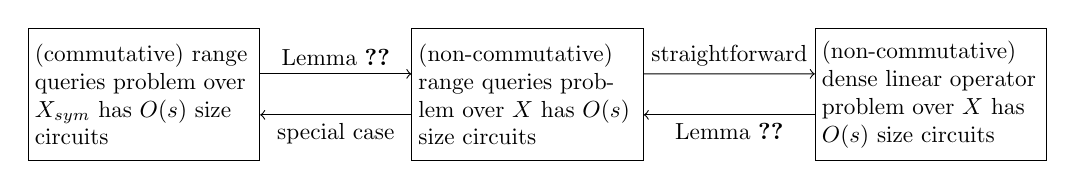
\begin{tikzpicture}[scale=0.84,transform shape]
%\draw[help lines] (0,0) grid (16,6);
\tikzstyle{v}=[rectangle,draw,inner sep=1mm,text width=33mm,above right,minimum height=20mm]

\node[v] (a) at (0,0) {(commutative) range queries problem over $X_{sym}$ has $O(s)$ size circuits};
\node[v] (b) at (5.8,0) {(non-commutative) range queries problem over $X$ has $O(s)$ size circuits};
\node[v] (c) at (11.9,0) {(non-commutative) dense linear operator problem over $X$ has $O(s)$ size circuits};

\path (a.10) edge[->] node[above] {Lemma~\ref{lem:intervals}} (b.170);
\path (b.190) edge[->] node[below] {special case} (a.-10);
\path (b.10) edge[->] node[above] {straightforward} (c.170);
\path (c.190) edge[->] node[below] {Lemma~\ref{lem:dense_matrices}} (b.-10);
\end{tikzpicture}
\end{center}
\vspace{2mm}

In these equivalences, non-commutative problems are considered over an arbitrary
strongly non-commutative semigroup and the commutative problem is considered
over free idempotent commutative semigroup $X_{sym}$. Recall that
if we factorize any strongly non-commutative idempotent semigroup over
commutativity equivalences, we obtain exactly free idempotent commutative
semigroup.

Note that two of the reductions on this diagram are trivial. The other two are
formulated in the following lemmas.

%To show the theorem we introduce an intermediate problem: computing non-commutative intervals by $O(n)$-size circuit.
%
%Clearly, this problem subsumes both of our problems. Indeed, if we can compute non-commutative intervals, we can compute commutative intervals by the same circuit.
%On the other hand, if we can compute non-commutative intervals, then given non-commutative dense matrix we can split it into intervals, compute them separately, then join them together in $O(n)$.
%
%Thus, it remains to show the following two lemmas.

\begin{lemma} \label{lem:dense_matrices}
If the (non-commutative) dense linear operator problem over $X$ has size $s$
circuit then the (non-commutative) range queries problem over $X$ has size
$O(s)$ circuit.
%If we can compute non-commutative dense matrices by a linear size circuit, we can also compute non-commutative intervals.
\end{lemma}

\begin{lemma} \label{lem:intervals}
If the (commutative) version of the range queries problem over $X_{sym}$ has
size $s$ circuits then the (non-commutative) version over $X$ also does.
%If we can compute commutative intervals by a linear size circuit, we can also compute non-commutative intervals.
\end{lemma}

The proofs of these lemmas are presented in
Sections~\ref{sec:operators_to_queries}
and~\ref{sec:non-commutative_to_commutative} respectively.

\input non_commutative_proofs

\section{Open Problems}
There are several natural problems left open.
\begin{enumerate}
\item Design a~deterministic $O(z)$ time algorithm for generating
a~circuit in the commutative case.
For this, it suffices to design an $O(n)$ deterministic algorithm for the
following problem: given a~list of positions of $n$~zeroes of an $n \times n$
0/1-matrix with at most $\log n$ zeroes in every row, permute its columns so
that the total length of all segments of length at most $O(\log n)$ is
$O(\frac{n}{\log n})$.
\item Determine the asymptotic complexity of the linear operator in terms of the number of zeroes in the non-commutative case.
\item After the preliminary version of our paper Stasys Jukna posed a question on how large can the gap between the complexity of the operators $Ax$ and $\overline{A}x$ can be over $(\mathbb{N},+)$ semiring, where $A \in \{0,1\}^{n\times n}$ and $\overline{A}$ is a bit-wise negation of $A$. Our result rules out the possibility of achieving super-constant (multiplicative) gap with sparse matrix $A$.

\end{enumerate}


\section*{Acknowledgments}
We thank Pawel Gawrychowski for pointing us to the
paper~\cite{DBLP:journals/ijcga/ChazelleR91}, and Alexey Talambutsa for
fruitful discussions on the theory of semigroups.
We are also grateful to the reviewers for their thorough reviews that helped us
improve the final version of the paper.

\clearpage

\appendix
\section{Review}
\input algebraic_structures
\input range_queries_applications
\input approaches
\input dense_graph_repr

\bibliographystyle{tocplain}
\bibliography{references}

%%% !!! AUTHOR
%%% Include a short description of each author's affiliation
%%% following the structure below. Use the same unique ID used
%%% previously (presumably lower case last name).
%%% Use \tocat{} and \tocdot{} instead of "@" and "." in emails
% \begin{tocinfo}[surname]
%     Firstname Surname\\
%     Assistant professor\\
%     Department of Computer Science and\\
%     Department of Immunology\\
%     Exemplar University\\
%     Town, State/Province, Country\\
%     name\tocat{}cs\tocdot{}exemplar\tocdot{}edu \\   %% email address here
%     \url{http://cs.exemplar.edu/~surname}      %% your home page here
%    \end{tocinfo}

\begin{tocauthors}
\begin{tocinfo}[kulikov]
    Alexander S. Kulikov\\
    Steklov Mathematical Institute at St.~Petersburg,     Russian Academy of~Sciences\\ and St.~Petersburg State University\\
    kulikov\tocat{}logic\tocdot{}pdmi\tocdot{}ras\tocdot{}ru\\
    \url{https://logic.pdmi.ras.ru/\~kulikov/}
\end{tocinfo}
\begin{tocinfo}[mikhailin]
    Ivan Mikhailin\\
    Steklov Mathematical Institute at St.~Petersburg,     Russian Academy of~Sciences\\
    ivmihajlin\tocat{}gmail\tocdot{}com
\end{tocinfo}
\begin{tocinfo}[mokhov]
    Andrey Mokhov\\
    School of Engineering, Newcastle University, United Kingdom\\
    andrey.mokhov\tocat{}ncl\tocdot{}ac\tocdot{}uk
\end{tocinfo}
\begin{tocinfo}[podolskii]
    Vladimir V. Podolskii\\
    Steklov Mathematical Institute\\
    Russian Academy of Sciences\\
    podolskii\tocat{}mi-ras\tocdot{}ru\\
    \url{http://www.mi-ras.ru/\~podolskii/}
\end{tocinfo}
\end{tocauthors}

\end{document}
